\title{RAID}
\maketitle
\tikzset{>=stealth,
  node distance=2.75cm,
  every node/.style={font=\footnotesize},
  disk/.style={
    cylinder,
    cylinder uses custom fill,
    cylinder body fill=yellow!50,
    cylinder end fill=yellow!50,
    shape border rotate=90,
    aspect=0.7,
    minimum height=1.4cm,
    minimum width=1cm,
    draw
  },
  rdisk/.style={disk, 
    cylinder body fill=blue!60,
    cylinder end fill=blue!60
  }
}

\section{\inserttitle}

\begin{frame}{\inserttitle}{Introdução}
  \begin{itemize}
  \item RAID ({\em Redundant Array of Inexpensive Disks}) -- em uma tradução livre, 
    arranjo redundante de discos de baixo custo.
  \item Objetivo: aumentar a confiabilidade e capacidade de armazenamento usando 
    discos de baixo custo.
  \item Este objetivo foi atingido graças ao paralelismo atingido
    pelos processadores, que permitiu várias operações de E/S
    simultâneas.
  \end{itemize}
\end{frame}

\begin{frame}{RAID 0}{Sem redundância}
  
  \begin{center}
    \begin{tikzpicture}
      \node[disk] (d0) {};
      \node[disk, right of=d0] (d1) {};
      \node[disk, right of=d1] (d2) {};
      \node[disk, right of=d2] (d3) {};
      
      \node[below of=d1, xshift=-3.5cm,yshift=1.25cm] (left) {};
      \node[below of=d1, xshift=6cm,yshift=1.25cm] (right) {};
      \path[thick,draw] (left) -- node[above] {discos de dados} node[blue,below] {discos de checagem e redundância} (right);
      
    \end{tikzpicture}
  \end{center}
\end{frame}

\begin{frame}{RAID 1}{Espelhamento}
  
  \begin{center}
    \begin{tikzpicture}
      \node[disk] (d0) {};
      \node[disk, right of=d0] (d1) {};
      \node[disk, right of=d1] (d2) {};
      \node[disk, right of=d2] (d3) {};
      
      \node[below of=d1, xshift=-3.5cm,yshift=1.25cm] (left) {};
      \node[below of=d1, xshift=6cm,yshift=1.25cm] (right) {};
      \path[thick,draw] (left) -- node[above] {discos de dados} node[blue,below] {discos de checagem e redundância} (right);
      
      \node[rdisk, below of=d0] (r0) {};
      \node[rdisk, below of=d1] (r1) {};
      \node[rdisk, below of=d2] (r2) {};
      \node[rdisk, below of=d3] (r3) {};
      
    \end{tikzpicture}
  \end{center}
\end{frame}

\begin{frame}{RAID 2}{Detecção de erro e correção de código}
  
  Não utilizado.

  \begin{center}
    \begin{tikzpicture}
      \node[disk] (d0) {};
      \node[disk, right of=d0] (d1) {};
      \node[disk, right of=d1] (d2) {};
      \node[disk, right of=d2] (d3) {};
      
      \node[below of=d1, xshift=-3.5cm,yshift=1.25cm] (left) {};
      \node[below of=d1, xshift=6cm,yshift=1.25cm] (right) {};
      \path[thick,draw] (left) -- node[above] {discos de dados} node[blue,below] {discos de checagem e redundância} (right);
      
      \node[rdisk, below of=d0] (r0) {};
      \node[rdisk, below of=d1] (r1) {};
      \node[rdisk, below of=d2] (r2) {};
    \end{tikzpicture}
  \end{center}
\end{frame}


\begin{frame}{RAID 3}{Paridade de bits}
  
  \begin{center}
    \begin{tikzpicture}
      \node[disk] (d0) {};
      \node[disk, right of=d0] (d1) {};
      \node[disk, right of=d1] (d2) {};
      \node[disk, right of=d2] (d3) {};
      
      \node[below of=d1, xshift=-3.5cm,yshift=1.25cm] (left) {};
      \node[below of=d1, xshift=6cm,yshift=1.25cm] (right) {};
      \path[thick,draw] (left) -- node[above] {discos de dados} node[blue,below] {discos de checagem e redundância} (right);
      
      \node[rdisk, below of=d0] (r0) {};
    \end{tikzpicture}
  \end{center}
\end{frame}


\begin{frame}{RAID 4}{Paridade de blocos}
  
  \begin{center}
    \begin{tikzpicture}
      \node[disk] (d0) {};
      \node[disk, right of=d0] (d1) {};
      \node[disk, right of=d1] (d2) {};
      \node[disk, right of=d2] (d3) {};
      
      \node[below of=d1, xshift=-3.5cm,yshift=1.25cm] (left) {};
      \node[below of=d1, xshift=6cm,yshift=1.25cm] (right) {};
      \path[thick,draw] (left) -- node[above] {discos de dados} node[blue,below] {discos de checagem e redundância} (right);
      
      \node[rdisk, below of=d0] (r0) {};
    \end{tikzpicture}
  \end{center}
\end{frame}

\begin{frame}{RAID 5}{Paridade de blocos distribuída}
  
  \begin{center}
    \begin{tikzpicture}
      \node[disk] (d0) {};
      \node[disk, right of=d0] (d1) {};
      \node[disk, right of=d1] (d2) {};
      \node[disk, right of=d2] (d3) {};
      
      \node[below of=d1, xshift=-3.5cm,yshift=1.25cm] (left) {};
      \node[below of=d1, xshift=6cm,yshift=1.25cm] (right) {};
      \path[thick,draw] (left) -- node[above] {discos de dados} node[blue,below] {discos de checagem e redundância} (right);
      
      \node[rdisk, below of=d0] (r0) {};
    \end{tikzpicture}
  \end{center}
\end{frame}


\begin{frame}{RAID 6}{Redundância com paridade dupla}
  
  \begin{center}
    \begin{tikzpicture}
      \node[disk] (d0) {};
      \node[disk, right of=d0] (d1) {};
      \node[disk, right of=d1] (d2) {};
      \node[disk, right of=d2] (d3) {};
      
      \node[below of=d1, xshift=-3.5cm,yshift=1.25cm] (left) {};
      \node[below of=d1, xshift=6cm,yshift=1.25cm] (right) {};
      \path[thick,draw] (left) -- node[above] {discos de dados} node[blue,below] {discos de checagem e redundância} (right);
      
      \node[rdisk, below of=d0] (r0) {};
      \node[rdisk, below of=d1] (r1) {};
    \end{tikzpicture}
  \end{center}
\end{frame}


%%%%%%%%%%%%%%%%%%%%%%%%%%%%%%%%%%%%%%%%%%%%%%%%%%%%%%%%%%%%%%%%
%% BUFFER
%%%%%%%%%%%%%%%%%%%%%%%%%%%%%%%%%%%%%%%%%%%%%%%%%%%%%%%%%%%%%%%%
\ifnum1=2

\lecture{RAID}

\begin{frame}{RAID 0}
  
  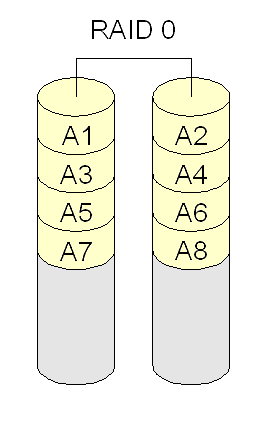
\includegraphics[scale=.3]{raid0.png}

\end{frame}


\begin{frame}{RAID 1}
  
  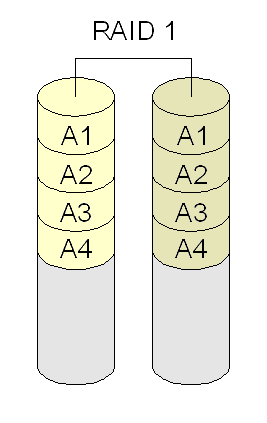
\includegraphics[scale=.3]{raid1.png}

\end{frame}


\begin{frame}{RAID 5}
  
  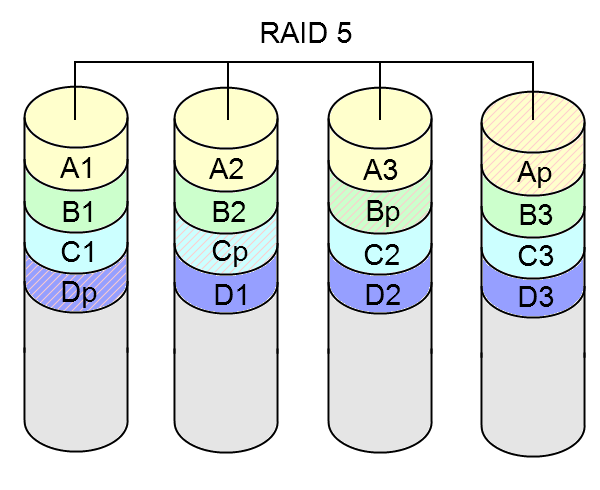
\includegraphics[scale=.3]{raid5.png}

\end{frame}

\begin{frame}{RAID 0+1}
  
  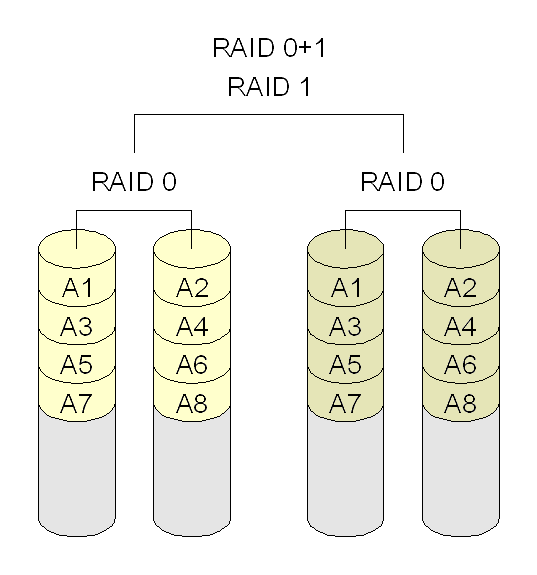
\includegraphics[scale=.3]{raid01.png}

\end{frame}

\fi